% --
% theory

\section{Theory}\label{sec:nn_theory}
\thesisStateNotReady
This section provides the preliminaries of theory to understand the used neural network architectures in their structure. 
Further the general training procedure of neural networks is explained.

% --
% activation functions

\subsection{Activation Functions}\label{sec:nn_theory_acti}
Activation functions for neural networks are non-linear functions that usually maps the sum of the weighted inputs of a node to a single output value $z$ as following:
\begin{equation}\label{eq:nn_theory_acti}
  z = h(w \, x^T)
\end{equation}
where $h$ is the activation function, $w \in \R^n$ is an weight vector and $x \in \R^n$ an input vector for one specific node.
The constraint of an activation function is, that an easy computable derivative of this function exist, in order to backpropagate gradients.

The most famous activation function nowadays is the RELU function:
\begin{equation}\label{eq:nn_theory_relu}
  z = \max{(0, a)}
\end{equation}
with $a \in \R$ as input to the activation function.
The big advantage is that this function and its subgradients are very easy and fast to compute.
The two other activation functions that are used in wavenets are the sigmoid function:
\begin{equation}\label{eq:nn_theory_sigmoid}
  z = 
\end{equation}
and the tanh functions:
\begin{equation}\label{eq:nn_theory_tanh}
  z = 
\end{equation}

% --
% fully connected

\subsection{Fully Connected Layer}
A fully connected (FC) layer is the simplest and most basic forms in neural networks.
Each node from the previous layer is connected in forward direction to all nodes in the FC layer and each node in the FC layer is further connected to all nodes in the next layer.
Further each connection has one trainable weight and each node has a bias term.
A simple FC layer is illustrated in \rfig{nn_theory_fc}.
% fc
\begin{figure}[!ht]
  \centering
    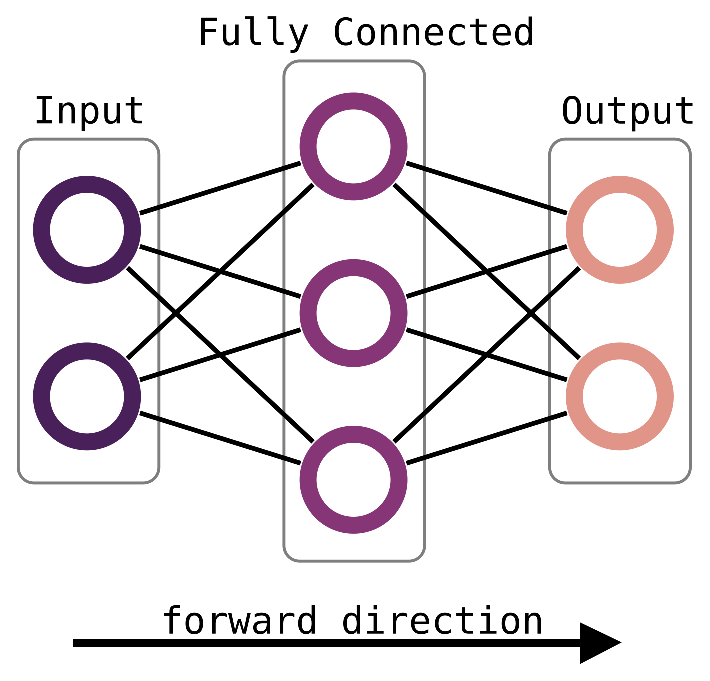
\includegraphics[width=0.35\textwidth]{./4_nn/figs/nn_theory_fc.eps}
  \caption{Basic fully connected layer with 3 nodes, receiving connections from 2 input nodes and outputing connections to 2 output nodes.}
  \label{fig:nn_theory_fc}
\end{figure}
\FloatBarrier
\noindent
In one node usually following computation is processed:
\begin{equation}
  z = h(w \, x^T + b)
\end{equation}
with the same notations as in \req{nn_theory_acti} and an additional bias term $b \in \R$.


% --
% cnn

\subsection{Convolutional Layers}\label{sec:nn_theory_cnn}
Convolutional layers are the fundament of every Covolutional Neural Networks (CNN) as already discussed in \rsec{prev_nn_cnn}.
They use convolutional filters on small areas of the input data, so that spatial information is retrieved.
Those convolutional filters are also called kernels and illustrated in case of images as rectangle in 2D space with kernel width $k_w$ and height $k_h$.
The kernel is shifted over its input map in each axis with an operation called \emph{stride}, denoted as $s$, and produce a output map through convolution.
The output dimension $o_d$ for striding along this axis with $s_d$ and kernel size for that axis $k_d$ over the input dimension $i_d$ can be computed as:
\begin{equation}\label{eq:nn_theory_cnn_}
  o_d = \floor*{\frac{i_d + p_d - k_d}{s_d} + 1}
\end{equation}
where $p_d$ is additionally a \emph{padding} term, where for instance for in zero-padding, zeros are added on both sides of the input dimension.
For example if a $16 \times 16$ image is convoluted by a $5 \times 5$ kernel with stride $1$ in each direction and no padding, the output image is $12 \times 12$.
The padding operation has usually the purpose to keep a the output and input dimension the same.
This is used for instance in residual neural networks, where the input to convolutional layers of a block, is bypassed and added to the output of this block again.
Being able to compute the addition operation from input and output of the residual block, their dimensions must be the same.
However in most convolutional network applications without residual blocks, it is preferred not to pad the image, so that dimensions are reduced hence parameters and multiplications saved.
Further there exist some special convolutional layers designed to reduce the dimensions (subsampling), such as a Max-Pooling layer. 

As already mentioned above CNNs are defined with the amount of input and output channels (feature maps), the kernel size, the stride of the kernel and some other specialties like dilation.
However it is not immediately clear from those parameter, how many convolutional filters are applied and what how the output feature maps are calculated exactly.
The amount of convolutional filters is in most practical examples always:
\begin{equation}\label{eq:nn_theory_n_filters}
  \#k = i \cdot j
\end{equation}
where $i$ and $j$ is the amount of input and output channels respectively.
Each kernel produces an output map, but the idea is to constraint the number of output maps $\#k$ to the defined output channels $j$.
This is usually done by summing up all output maps of input channels $i$ for one output channel $j$:
\begin{equation}
  o_j = \sum_{i} k_{i, j} * x_i
\end{equation}
where $o_j$ is the j-th feature map, $k_{i, j}$ the kernel of $i$ and $j$ and $x_i$ the i-th input channel.
A gaphical example of this procedure is shown in \rfig{nn_theory_cnn_basics}.

\begin{figure}[!ht]
  \centering
    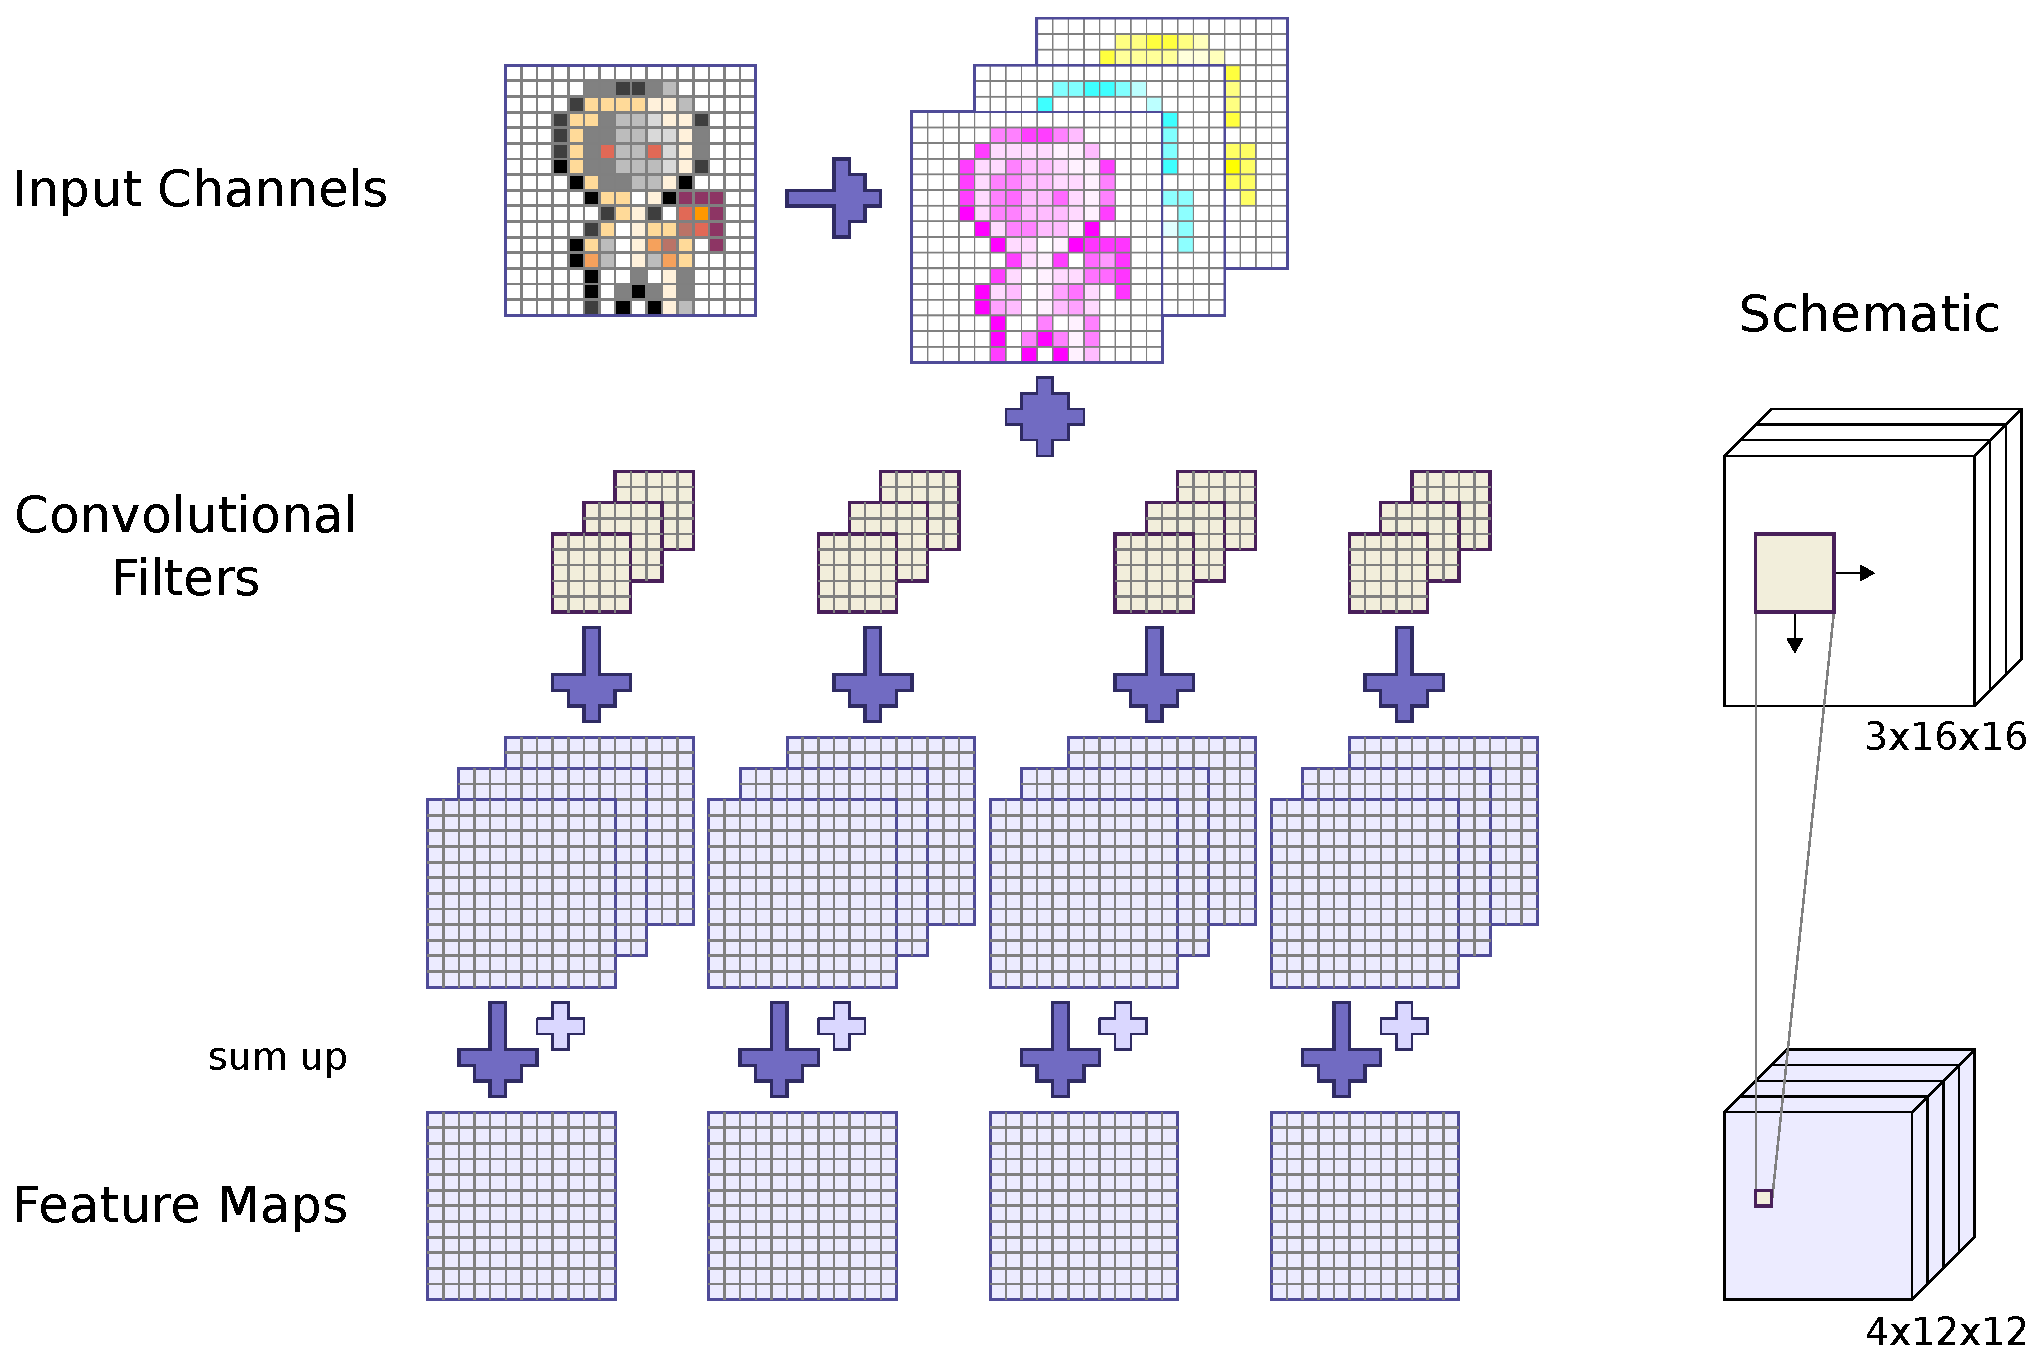
\includegraphics[width=0.6\textwidth]{./4_nn/figs/nn_theory_cnn_basics.eps}
  \caption{Basic CNN layer with a $16 \times 16$ input image, decomposed in 3 channels (CYM) and 4 output feature maps. Kernel size is $5 \times 5$ and the stride is $1$.}
  \label{fig:nn_theory_cnn_basics}
\end{figure}
\FloatBarrier
\noindent

% \begin{figure}[h]
%   \centering{
%   \resizebox{0.5\textwidth}{!}{\input{./4_nn/figs/cnn_basics.tex}}}
%   \caption{CNN basic architecture}
%   \label{fig:nn_theory_cnn_basic}
% \end{figure}
% \FloatBarrier
% \noindent


